% generated by GAPDoc2LaTeX from XML source (Frank Luebeck)
\documentclass[a4paper,11pt]{report}

\usepackage{a4wide}
\sloppy
\pagestyle{myheadings}
\usepackage{amssymb}
\usepackage[utf8]{inputenc}
\usepackage{makeidx}
\makeindex
\usepackage{color}
\definecolor{FireBrick}{rgb}{0.5812,0.0074,0.0083}
\definecolor{RoyalBlue}{rgb}{0.0236,0.0894,0.6179}
\definecolor{RoyalGreen}{rgb}{0.0236,0.6179,0.0894}
\definecolor{RoyalRed}{rgb}{0.6179,0.0236,0.0894}
\definecolor{LightBlue}{rgb}{0.8544,0.9511,1.0000}
\definecolor{Black}{rgb}{0.0,0.0,0.0}

\definecolor{linkColor}{rgb}{0.0,0.0,0.554}
\definecolor{citeColor}{rgb}{0.0,0.0,0.554}
\definecolor{fileColor}{rgb}{0.0,0.0,0.554}
\definecolor{urlColor}{rgb}{0.0,0.0,0.554}
\definecolor{promptColor}{rgb}{0.0,0.0,0.589}
\definecolor{brkpromptColor}{rgb}{0.589,0.0,0.0}
\definecolor{gapinputColor}{rgb}{0.589,0.0,0.0}
\definecolor{gapoutputColor}{rgb}{0.0,0.0,0.0}

%%  for a long time these were red and blue by default,
%%  now black, but keep variables to overwrite
\definecolor{FuncColor}{rgb}{0.0,0.0,0.0}
%% strange name because of pdflatex bug:
\definecolor{Chapter }{rgb}{0.0,0.0,0.0}
\definecolor{DarkOlive}{rgb}{0.1047,0.2412,0.0064}


\usepackage{fancyvrb}

\usepackage{mathptmx,helvet}
\usepackage[T1]{fontenc}
\usepackage{textcomp}


\usepackage[
            pdftex=true,
            bookmarks=true,        
            a4paper=true,
            pdftitle={Written with GAPDoc},
            pdfcreator={LaTeX with hyperref package / GAPDoc},
            colorlinks=true,
            backref=page,
            breaklinks=true,
            linkcolor=linkColor,
            citecolor=citeColor,
            filecolor=fileColor,
            urlcolor=urlColor,
            pdfpagemode={UseNone}, 
           ]{hyperref}

\newcommand{\maintitlesize}{\fontsize{50}{55}\selectfont}

% write page numbers to a .pnr log file for online help
\newwrite\pagenrlog
\immediate\openout\pagenrlog =\jobname.pnr
\immediate\write\pagenrlog{PAGENRS := [}
\newcommand{\logpage}[1]{\protect\write\pagenrlog{#1, \thepage,}}
%% were never documented, give conflicts with some additional packages

\newcommand{\GAP}{\textsf{GAP}}

%% nicer description environments, allows long labels
\usepackage{enumitem}
\setdescription{style=nextline}

%% depth of toc
\setcounter{tocdepth}{1}

\usepackage{amsmath}\usepackage[T1]{fontenc}
\usepackage{tikz}
\usetikzlibrary{shapes,arrows,matrix}
\usepackage{faktor}



%% command for ColorPrompt style examples
\newcommand{\gapprompt}[1]{\color{promptColor}{\bfseries #1}}
\newcommand{\gapbrkprompt}[1]{\color{brkpromptColor}{\bfseries #1}}
\newcommand{\gapinput}[1]{\color{gapinputColor}{#1}}


\begin{document}

\logpage{[ 0, 0, 0 ]}
\begin{titlepage}
\mbox{}\vfill

\begin{center}{\maintitlesize \textbf{ Bicomplexes \mbox{}}}\\
\vfill

\hypersetup{pdftitle= Bicomplexes }
\markright{\scriptsize \mbox{}\hfill  Bicomplexes  \hfill\mbox{}}
{\Huge \textbf{ Bicomplexes for Abelian categories \mbox{}}}\\
\vfill

{\Huge  2017.05.02 \mbox{}}\\[1cm]
{ 2 May 2017 \mbox{}}\\[1cm]
\mbox{}\\[2cm]
{\Large \textbf{ Mohamed Barakat\\
    \mbox{}}}\\
{\Large \textbf{ Kamal Saleh\\
    \mbox{}}}\\
\hypersetup{pdfauthor= Mohamed Barakat\\
    ;  Kamal Saleh\\
    }
\end{center}\vfill

\mbox{}\\
{\mbox{}\\
\small \noindent \textbf{ Mohamed Barakat\\
    }  Email: \href{mailto://mohamed.barakat@uni-siegen.de} {\texttt{mohamed.barakat@uni-siegen.de}}\\
  Homepage: \href{http://www.mathematik.uni-kl.de/~barakat/} {\texttt{http://www.mathematik.uni-kl.de/\texttt{\symbol{126}}barakat/}}\\
  Address: \begin{minipage}[t]{8cm}\noindent
 Walter-Flex-Str. 3\\
 57068 Siegen\\
 Germany\\
 \end{minipage}
}\\
{\mbox{}\\
\small \noindent \textbf{ Kamal Saleh\\
    }  Email: \href{mailto://kamal.saleh@uni-siegen.de} {\texttt{kamal.saleh@uni-siegen.de}}\\
  Homepage: \href{https://github.com/kamalsaleh/} {\texttt{https://github.com/kamalsaleh/}}\\
  Address: \begin{minipage}[t]{8cm}\noindent
 Walter-Flex-Str. 3\\
 57068 Siegen\\
 Germany\\
 \end{minipage}
}\\
\end{titlepage}

\newpage\setcounter{page}{2}
\newpage

\def\contentsname{Contents\logpage{[ 0, 0, 1 ]}}

\tableofcontents
\newpage

     
\chapter{\textcolor{Chapter }{Bicomplexes}}\label{Chapter_Bicomplexes}
\logpage{[ 1, 0, 0 ]}
\hyperdef{L}{X7CEDAD61826170CF}{}
{
  

  Let us create the following chain complex of chain complexes of left
presentations over $\mathbb{Z}$: \begin{center} 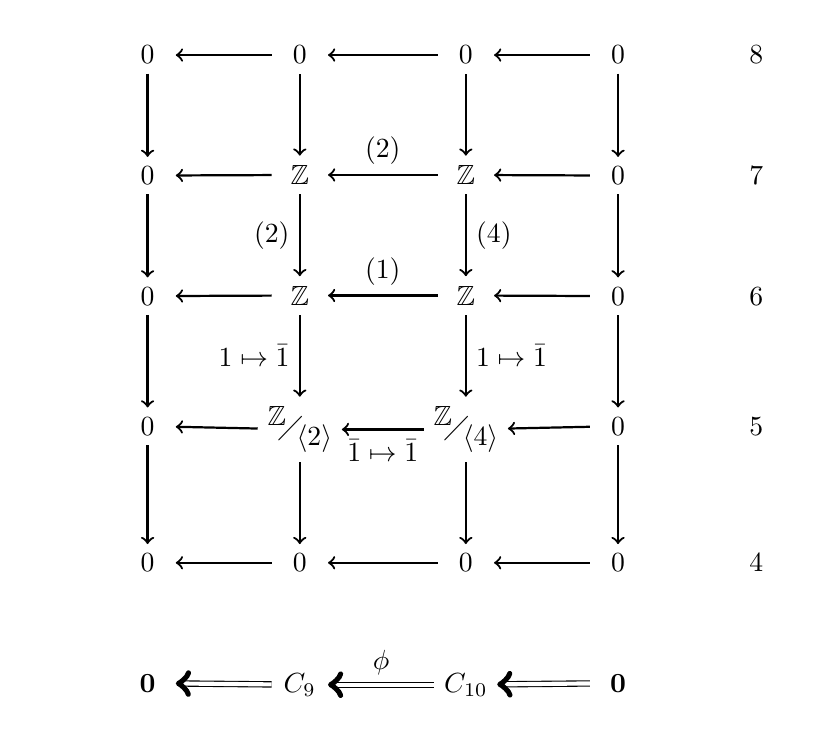
\begin{tikzpicture} \matrix
(m) [matrix of math nodes,row sep=3em,column sep=3em,minimum width=2em] { & 0
& 0 & 0 & 0 & 8 \\ & 0 & \mathbb{Z} & \mathbb{Z} & 0 & 7 \\ & 0 & \mathbb{Z} &
\mathbb{Z} & 0 & 6 \\ & 0 & \faktor{\mathbb{Z}}{\langle 2 \rangle} &
\faktor{\mathbb{Z}}{\langle 4 \rangle} & 0 & 5 \\ & 0 & 0 & 0 & 0 & 4 \\
&\mathbf{0} & C_9 & C_{10} & \mathbf{0} &\\}; \path[-stealth] (m-2-2) edge[
<-,thick] (m-2-3) (m-2-2) edge[ ->,thick] (m-3-2) (m-3-2) edge[ ->,thick]
(m-4-2) (m-1-2) edge[ ->,thick] (m-2-2) (m-1-5) edge[ ->,thick] (m-2-5)
(m-2-3) edge[ <-,thick] node[above]{$(2)$} (m-2-4) (m-1-3) edge[ <-,thick]
(m-1-4) (m-1-2) edge[ <-,thick] (m-1-3) (m-2-4) edge[ <-,thick] (m-2-5)
(m-3-2) edge[ <-,thick] (m-3-3) (m-1-4) edge[ <-,thick] (m-1-5) (m-3-3) edge[
<-,thick] node[above]{$(1)$} (m-3-4) (m-3-4) edge[ <-,thick] (m-3-5) (m-2-3)
edge[ <-,thick] (m-1-3) (m-2-4) edge[ <-,thick] (m-1-4) (m-3-3) edge[
<-,thick] node[left]{$(2)$} (m-2-3) (m-3-4) edge[ <-,thick] node[right]{$(4)$}
(m-2-4) (m-3-5) edge[ <-,thick] (m-2-5) (m-4-5) edge[ <-,thick] (m-3-5)
(m-4-3) edge[ <-,thick] node[left]{$1\mapsto \bar{1}$} (m-3-3) (m-4-4) edge[
<-,thick] node[right]{$1\mapsto \bar{1}$} (m-3-4) (m-5-4) edge[ <-,thick]
(m-4-4) (m-5-3) edge[ <-,thick] (m-4-3) (m-4-2) edge[ <-,thick] (m-4-3)
(m-4-3) edge[ <-,thick] node[below]{$\bar{1}\mapsto \bar{1}$} (m-4-4) (m-4-4)
edge[ <-,thick] (m-4-5) (m-5-4) edge[ <-,thick] (m-5-5) (m-5-3) edge[
<-,thick] (m-5-4) (m-5-2) edge[ <-,thick] (m-5-3) (m-5-2) edge[ <-,thick]
(m-4-2) (m-5-5) edge[ <-,thick] (m-4-5) (m-6-4) edge[ double distance =
1.5pt,<-,thin] (m-6-5) (m-6-3) edge[ double distance = 1.5pt,<-,thin]
node[above]{$\phi$} (m-6-4) (m-6-2) edge[ double distance = 1.5pt,<-,thin]
(m-6-3) ; \end{tikzpicture} \end{center}  
\begin{Verbatim}[commandchars=!@|,fontsize=\small,frame=single,label=Example]
  !gapprompt@gap>| !gapinput@ZZ := HomalgRingOfIntegers( );|
  Z
  !gapprompt@gap>| !gapinput@lp_cat := CategoryOfHomalgLeftModules( ZZ );|
  intrinsic Category of left presentations of Z with ambient objects
  !gapprompt@gap>| !gapinput@chains_lp_cat := ChainComplexCategory( lp_cat );|
  Chain complexes category over intrinsic Category
  of left presentations of Z with ambient objects
  !gapprompt@gap>| !gapinput@chains_chains_lp_cat := ChainComplexCategory( chains_lp_cat );|
  Chain complexes category over chain complexes category over
  intrinsic Category of left presentations of Z with ambient objects
  !gapprompt@gap>| !gapinput@Bicomplexes_cat := AsCategoryOfBicomplexes( chains_chains_lp_cat );|
  Chain complexes category over chain complexes category over
  intrinsic Category of left presentations of Z with ambient objects
  as bicomplexes
  !gapprompt@gap>| !gapinput@F1 := HomalgFreeLeftModule( 1, ZZ );|
  <A free left module of rank 1 on a free generator>
  !gapprompt@gap>| !gapinput@d7 := HomalgMap( HomalgMatrix( "[ [ 4 ] ]", 1, 1, ZZ ), F1, F1 );|
  <An endo"morphism" of a left module>
  !gapprompt@gap>| !gapinput@d6 := CokernelProjection( d7 );|
  <An epimorphism of left modules>
  !gapprompt@gap>| !gapinput@C10 := ChainComplex( [ d6, d7 ], 6 );|
  <A bounded object in chain complexes category over intrinsic 
  Category of left presentations of Z with ambient objects with 
  active lower bound 4 and active upper bound 8>
  !gapprompt@gap>| !gapinput@t7 := HomalgMap( HomalgMatrix( "[ [ 2 ] ]", 1, 1, ZZ ), F1, F1 );|
  <An endo"morphism" of a left module>
  !gapprompt@gap>| !gapinput@t6 := CokernelProjection( t7 );|
  <An epimorphism of left modules>
  !gapprompt@gap>| !gapinput@C9 := ChainComplex( [ t6, t7 ], 6 );|
  <A bounded object in chain complexes category over intrinsic 
  Category of left presentations of Z with ambient objects with 
  active lower bound 4 and active upper bound 8>
  !gapprompt@gap>| !gapinput@phi5 := HomalgMap( HomalgIdentityMatrix( 1, ZZ ), C10[ 5 ], C9[ 5 ] );|
  <A "homomorphism" of left modules>
  !gapprompt@gap>| !gapinput@phi6 := HomalgMap( HomalgIdentityMatrix( 1, ZZ ), F1, F1 );|
  <An endo"morphism" of a left module>
  !gapprompt@gap>| !gapinput@phi7 := HomalgMap( 2 * HomalgIdentityMatrix( 1, ZZ ), F1, F1 );|
  <An endo"morphism" of a left module>
  !gapprompt@gap>| !gapinput@phi := ChainMorphism( C10, C9, [ phi5, phi6, phi7 ], 5 );|
  <A bounded morphism in chain complexes category over intrinsic 
  Category of left presentations of Z with ambient objects with 
  active lower bound 4 and active upper bound 8>
  !gapprompt@gap>| !gapinput@C := ChainComplex( [ phi ], 10 );|
  <A bounded object in chain complexes category over chain complexes 
  category over intrinsic Category of left presentations of Z with 
  ambient objects with active lower bound 8 and active upper bound 11>
\end{Verbatim}
  Now we compute its associated homological bicomplex $B$ and the total complex
of $B$: \begin{center} 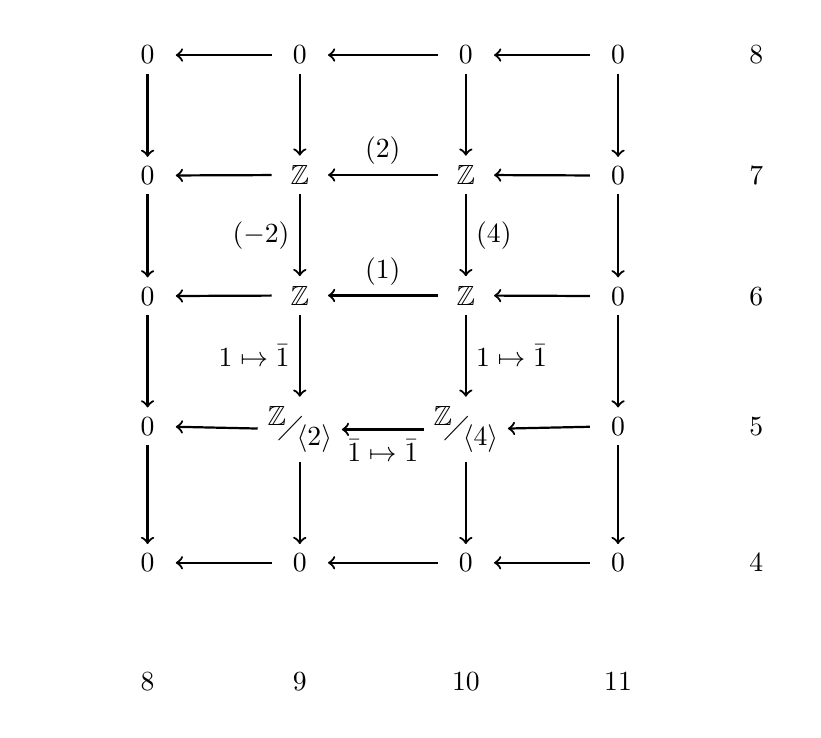
\begin{tikzpicture} \matrix (m) [matrix of math
nodes,row sep=3em,column sep=3em,minimum width=2em] { & 0 & 0 & 0 & 0 & 8 \\ &
0 & \mathbb{Z} & \mathbb{Z} & 0 & 7 \\ & 0 & \mathbb{Z} & \mathbb{Z} & 0 & 6
\\ & 0 & \faktor{\mathbb{Z}}{\langle 2 \rangle} & \faktor{\mathbb{Z}}{\langle
4 \rangle} & 0 & 5 \\ & 0 & 0 & 0 & 0 & 4 \\ & 8 & 9 & 10 & 11 &\\};
\path[-stealth] (m-2-2) edge[ <-,thick] (m-2-3) (m-2-2) edge[ ->,thick]
(m-3-2) (m-3-2) edge[ ->,thick] (m-4-2) (m-1-2) edge[ ->,thick] (m-2-2)
(m-1-5) edge[ ->,thick] (m-2-5) (m-2-3) edge[ <-,thick] node[above]{$(2)$}
(m-2-4) (m-1-3) edge[ <-,thick] (m-1-4) (m-1-2) edge[ <-,thick] (m-1-3)
(m-2-4) edge[ <-,thick] (m-2-5) (m-3-2) edge[ <-,thick] (m-3-3) (m-1-4) edge[
<-,thick] (m-1-5) (m-3-3) edge[ <-,thick] node[above]{$(1)$} (m-3-4) (m-3-4)
edge[ <-,thick] (m-3-5) (m-2-3) edge[ <-,thick] (m-1-3) (m-2-4) edge[
<-,thick] (m-1-4) (m-3-3) edge[ <-,thick] node[left]{$(-2)$} (m-2-3) (m-3-4)
edge[ <-,thick] node[right]{$(4)$} (m-2-4) (m-3-5) edge[ <-,thick] (m-2-5)
(m-4-5) edge[ <-,thick] (m-3-5) (m-4-3) edge[ <-,thick] node[left]{$1\mapsto
\bar{1}$} (m-3-3) (m-4-4) edge[ <-,thick] node[right]{$1\mapsto \bar{1}$}
(m-3-4) (m-5-4) edge[ <-,thick] (m-4-4) (m-5-3) edge[ <-,thick] (m-4-3)
(m-4-2) edge[ <-,thick] (m-4-3) (m-4-3) edge[ <-,thick]
node[below]{$\bar{1}\mapsto \bar{1}$} (m-4-4) (m-4-4) edge[ <-,thick] (m-4-5)
(m-5-4) edge[ <-,thick] (m-5-5) (m-5-3) edge[ <-,thick] (m-5-4) (m-5-2) edge[
<-,thick] (m-5-3) (m-5-2) edge[ <-,thick] (m-4-2) (m-5-5) edge[ <-,thick]
(m-4-5) ; \end{tikzpicture} \end{center}  
\begin{Verbatim}[commandchars=!@|,fontsize=\small,frame=single,label=Example]
  !gapprompt@gap>| !gapinput@B := HomologicalBicomplex( C );|
  <A homological bicomplex in intrinsic Category of left presentations 
  of Z with ambient objects concentrated in window [ 8 .. 11 ] x [ 4 .. 8 ]>
  !gapprompt@gap>| !gapinput@Display( VerticalDifferentialAt( B, 9, 7 ) );|
  [ [  -2 ] ]
  
  the map is currently represented by the above 1 x 1 matrix
  !gapprompt@gap>| !gapinput@T := TotalComplex( B );|
  <A bounded object in chain complexes category over intrinsic Category 
  of left presentations of Z with ambient objects with active lower 
  bound 13 and active upper bound 18>
  !gapprompt@gap>| !gapinput@T[ 13 ];|
  <A zero left module>
  !gapprompt@gap>| !gapinput@T[ 14 ];|
  <A cyclic torsion left module presented by 1 relation
   for a cyclic generator>
  !gapprompt@gap>| !gapinput@T[ 15 ];|
  <A non-torsion left module presented by 1 relation for 2 generators>
  !gapprompt@gap>| !gapinput@T[ 16 ];|
  <A free left module of rank 2 on free generators>
  !gapprompt@gap>| !gapinput@T[ 17 ];|
  <A free left module of rank 1 on a free generator>
  !gapprompt@gap>| !gapinput@T[ 18 ];|
  <A zero left module>
  !gapprompt@gap>| !gapinput@Display( T^16 );|
  [ [  -2,   0 ],
    [   1,   1 ] ]
  
  the map is currently represented by the above 2 x 2 matrix
  !gapprompt@gap>| !gapinput@IsExact( T );|
  true
  !gapprompt@gap>| !gapinput@T;|
  <A cyclic, bounded object in chain complexes category over intrinsic 
  Category of left presentations of Z with ambient objects with active 
  lower bound 13 and active upper bound 18>
  !gapprompt@gap>| !gapinput@Display( T, 13, 18 );|
  
  -----------------------------------------------------------------
  In index 13
  
  Object is
  0
  
  Differential is
  (an empty 0 x 0 matrix)
  
  the map is currently represented by the above 0 x 0 matrix
  
  -----------------------------------------------------------------
  In index 14
  
  Object is
  Z/< 2 > 
  
  Differential is
  (an empty 1 x 0 matrix)
  
  the map is currently represented by the above 1 x 0 matrix
  
  -----------------------------------------------------------------
  In index 15
  
  Object is
  [ [  0,  4 ] ]
  
  Cokernel of the map
  
  Z^(1x1) --> Z^(1x2),
  
  currently represented by the above matrix
  
  Differential is
  [ [  -1 ],
    [   1 ] ]
  
  the map is currently represented by the above 2 x 1 matrix
  
  -----------------------------------------------------------------
  In index 16
  
  Object is
  Z^(1 x 2)
  
  Differential is
  [ [  -2,   0 ],
    [   1,   1 ] ]
  
  the map is currently represented by the above 2 x 2 matrix
  
  -----------------------------------------------------------------
  In index 17
  
  Object is
  Z^(1 x 1)
  
  Differential is
  [ [  2,  4 ] ]
  
  the map is currently represented by the above 1 x 2 matrix
  
  -----------------------------------------------------------------
  In index 18
  
  Object is
  0
  
  Differential is
  (an empty 0 x 1 matrix)
  
  the map is currently represented by the above 0 x 1 matrix
\end{Verbatim}
 
\section{\textcolor{Chapter }{Categories}}\label{Chapter_Bicomplexes_Section_Categories}
\logpage{[ 1, 1, 0 ]}
\hyperdef{L}{X7CC6903E78F24167}{}
{
  

\subsection{\textcolor{Chapter }{IsCapCategoryBicomplexCell (for IsCapCategoryCell andIsAttributeStoringRep)}}
\logpage{[ 1, 1, 1 ]}\nobreak
\hyperdef{L}{X84CBFFF580D63EDC}{}
{\noindent\textcolor{FuncColor}{$\triangleright$\ \ \texttt{IsCapCategoryBicomplexCell({\mdseries\slshape arg})\index{IsCapCategoryBicomplexCell@\texttt{IsCapCategoryBicomplexCell}!for IsCapCategoryCell andIsAttributeStoringRep}
\label{IsCapCategoryBicomplexCell:for IsCapCategoryCell andIsAttributeStoringRep}
}\hfill{\scriptsize (filter)}}\\
\textbf{\indent Returns:\ }
\texttt{true} or \texttt{false} 



 The \textsf{GAP} category of cells in a \textsf{CAP} category of bicomplexes. }

 

\subsection{\textcolor{Chapter }{IsCapCategoryBicomplexObject (for IsCapCategoryBicomplexCell andIsCapCategoryObject)}}
\logpage{[ 1, 1, 2 ]}\nobreak
\hyperdef{L}{X7A225A8C815B4456}{}
{\noindent\textcolor{FuncColor}{$\triangleright$\ \ \texttt{IsCapCategoryBicomplexObject({\mdseries\slshape arg})\index{IsCapCategoryBicomplexObject@\texttt{IsCapCategoryBicomplexObject}!for IsCapCategoryBicomplexCell andIsCapCategoryObject}
\label{IsCapCategoryBicomplexObject:for IsCapCategoryBicomplexCell andIsCapCategoryObject}
}\hfill{\scriptsize (filter)}}\\
\textbf{\indent Returns:\ }
\texttt{true} or \texttt{false} 



 The \textsf{GAP} category of bicomplex objects in a \textsf{CAP} category of bicomplexes. }

 

\subsection{\textcolor{Chapter }{IsCapCategoryHomologicalBicomplexObject (for IsCapCategoryBicomplexObject)}}
\logpage{[ 1, 1, 3 ]}\nobreak
\hyperdef{L}{X82480AED7A67D01D}{}
{\noindent\textcolor{FuncColor}{$\triangleright$\ \ \texttt{IsCapCategoryHomologicalBicomplexObject({\mdseries\slshape arg})\index{IsCapCategoryHomologicalBicomplexObject@\texttt{IsCap}\-\texttt{Category}\-\texttt{Homological}\-\texttt{Bicomplex}\-\texttt{Object}!for IsCapCategoryBicomplexObject}
\label{IsCapCategoryHomologicalBicomplexObject:for IsCapCategoryBicomplexObject}
}\hfill{\scriptsize (filter)}}\\
\textbf{\indent Returns:\ }
\texttt{true} or \texttt{false} 



 The \textsf{GAP} category of homological bicomplex objects in a \textsf{CAP} category of bicomplexes. }

 

\subsection{\textcolor{Chapter }{IsCapCategoryCohomologicalBicomplexObject (for IsCapCategoryBicomplexObject)}}
\logpage{[ 1, 1, 4 ]}\nobreak
\hyperdef{L}{X7F2D3C91805A5030}{}
{\noindent\textcolor{FuncColor}{$\triangleright$\ \ \texttt{IsCapCategoryCohomologicalBicomplexObject({\mdseries\slshape arg})\index{IsCapCategoryCohomologicalBicomplexObject@\texttt{IsCap}\-\texttt{Category}\-\texttt{Cohomological}\-\texttt{Bicomplex}\-\texttt{Object}!for IsCapCategoryBicomplexObject}
\label{IsCapCategoryCohomologicalBicomplexObject:for IsCapCategoryBicomplexObject}
}\hfill{\scriptsize (filter)}}\\
\textbf{\indent Returns:\ }
\texttt{true} or \texttt{false} 



 The \textsf{GAP} category of cohomological bicomplex objects in a \textsf{CAP} category of bicomplexes. }

 

\subsection{\textcolor{Chapter }{IsCapCategoryBicomplexMorphism (for IsCapCategoryBicomplexCell andIsCapCategoryMorphism)}}
\logpage{[ 1, 1, 5 ]}\nobreak
\hyperdef{L}{X7B5DFA2682ADF118}{}
{\noindent\textcolor{FuncColor}{$\triangleright$\ \ \texttt{IsCapCategoryBicomplexMorphism({\mdseries\slshape arg})\index{IsCapCategoryBicomplexMorphism@\texttt{IsCapCategoryBicomplexMorphism}!for IsCapCategoryBicomplexCell andIsCapCategoryMorphism}
\label{IsCapCategoryBicomplexMorphism:for IsCapCategoryBicomplexCell andIsCapCategoryMorphism}
}\hfill{\scriptsize (filter)}}\\
\textbf{\indent Returns:\ }
\texttt{true} or \texttt{false} 



 The \textsf{GAP} category of bicomplex morphisms in a \textsf{CAP} category of bicomplexes. }

 

\subsection{\textcolor{Chapter }{IsCapCategoryHomologicalBicomplexMorphism (for IsCapCategoryBicomplexMorphism)}}
\logpage{[ 1, 1, 6 ]}\nobreak
\hyperdef{L}{X7FECBADB7FED3C1F}{}
{\noindent\textcolor{FuncColor}{$\triangleright$\ \ \texttt{IsCapCategoryHomologicalBicomplexMorphism({\mdseries\slshape arg})\index{IsCapCategoryHomologicalBicomplexMorphism@\texttt{IsCap}\-\texttt{Category}\-\texttt{Homological}\-\texttt{Bicomplex}\-\texttt{Morphism}!for IsCapCategoryBicomplexMorphism}
\label{IsCapCategoryHomologicalBicomplexMorphism:for IsCapCategoryBicomplexMorphism}
}\hfill{\scriptsize (filter)}}\\
\textbf{\indent Returns:\ }
\texttt{true} or \texttt{false} 



 The \textsf{GAP} category of homological bicomplex morphisms in a \textsf{CAP} category of bicomplexes. }

 

\subsection{\textcolor{Chapter }{IsCapCategoryCohomologicalBicomplexMorphism (for IsCapCategoryBicomplexMorphism)}}
\logpage{[ 1, 1, 7 ]}\nobreak
\hyperdef{L}{X7EC396067E8B1647}{}
{\noindent\textcolor{FuncColor}{$\triangleright$\ \ \texttt{IsCapCategoryCohomologicalBicomplexMorphism({\mdseries\slshape arg})\index{IsCapCategoryCohomologicalBicomplexMorphism@\texttt{IsCap}\-\texttt{Category}\-\texttt{Cohomological}\-\texttt{Bicomplex}\-\texttt{Morphism}!for IsCapCategoryBicomplexMorphism}
\label{IsCapCategoryCohomologicalBicomplexMorphism:for IsCapCategoryBicomplexMorphism}
}\hfill{\scriptsize (filter)}}\\
\textbf{\indent Returns:\ }
\texttt{true} or \texttt{false} 



 The \textsf{GAP} category of cohomological bicomplex morphisms in a \textsf{CAP} category of bicomplexes. }

 }

 
\section{\textcolor{Chapter }{Constructors}}\label{Chapter_Bicomplexes_Section_Constructors}
\logpage{[ 1, 2, 0 ]}
\hyperdef{L}{X86EC0F0A78ECBC10}{}
{
  

\subsection{\textcolor{Chapter }{AssociatedBicomplexObject (for IsChainOrCochainComplex)}}
\logpage{[ 1, 2, 1 ]}\nobreak
\label{AssociatedBicomplex_obj}
\hyperdef{L}{X79D66C8A838BC9C2}{}
{\noindent\textcolor{FuncColor}{$\triangleright$\ \ \texttt{AssociatedBicomplexObject({\mdseries\slshape cx})\index{AssociatedBicomplexObject@\texttt{AssociatedBicomplexObject}!for IsChainOrCochainComplex}
\label{AssociatedBicomplexObject:for IsChainOrCochainComplex}
}\hfill{\scriptsize (attribute)}}\\
\textbf{\indent Returns:\ }
a \textsf{CAP} object 



 Return the bicomplex associated to the complex of complexes \mbox{\texttt{\mdseries\slshape cx}}. }

 

\subsection{\textcolor{Chapter }{AssociatedBicomplexMorphism (for IsChainOrCochainMorphism)}}
\logpage{[ 1, 2, 2 ]}\nobreak
\label{AssociatedBicomplex_mor}
\hyperdef{L}{X7B39940985505A52}{}
{\noindent\textcolor{FuncColor}{$\triangleright$\ \ \texttt{AssociatedBicomplexMorphism({\mdseries\slshape mu})\index{AssociatedBicomplexMorphism@\texttt{AssociatedBicomplexMorphism}!for IsChainOrCochainMorphism}
\label{AssociatedBicomplexMorphism:for IsChainOrCochainMorphism}
}\hfill{\scriptsize (attribute)}}\\
\textbf{\indent Returns:\ }
a \textsf{CAP} morphism 



 Return the morphism of bicomplexes associated to the chain morphism between
two complexes of complexes \mbox{\texttt{\mdseries\slshape mu}}. }

 

\subsection{\textcolor{Chapter }{AssociatedBicomplexFunctor (for IsCapFunctor, IsString)}}
\logpage{[ 1, 2, 3 ]}\nobreak
\label{AssociatedBicomplex_fun}
\hyperdef{L}{X7F3AE9F287867A00}{}
{\noindent\textcolor{FuncColor}{$\triangleright$\ \ \texttt{AssociatedBicomplexFunctor({\mdseries\slshape F, name})\index{AssociatedBicomplexFunctor@\texttt{AssociatedBicomplexFunctor}!for IsCapFunctor, IsString}
\label{AssociatedBicomplexFunctor:for IsCapFunctor, IsString}
}\hfill{\scriptsize (operation)}}\\
\noindent\textcolor{FuncColor}{$\triangleright$\ \ \texttt{AssociatedBicomplexFunctor({\mdseries\slshape F})\index{AssociatedBicomplexFunctor@\texttt{AssociatedBicomplexFunctor}!for IsCapFunctor}
\label{AssociatedBicomplexFunctor:for IsCapFunctor}
}\hfill{\scriptsize (attribute)}}\\
\textbf{\indent Returns:\ }
a \textsf{CAP} functor 



 

 }

 

\subsection{\textcolor{Chapter }{AssociatedBicomplex (for IsCapNaturalTransformation, IsString)}}
\logpage{[ 1, 2, 4 ]}\nobreak
\label{AssociatedBicomplex_ntr}
\hyperdef{L}{X827932218253241C}{}
{\noindent\textcolor{FuncColor}{$\triangleright$\ \ \texttt{AssociatedBicomplex({\mdseries\slshape eta, name})\index{AssociatedBicomplex@\texttt{AssociatedBicomplex}!for IsCapNaturalTransformation, IsString}
\label{AssociatedBicomplex:for IsCapNaturalTransformation, IsString}
}\hfill{\scriptsize (operation)}}\\
\noindent\textcolor{FuncColor}{$\triangleright$\ \ \texttt{AssociatedBicomplex({\mdseries\slshape eta})\index{AssociatedBicomplex@\texttt{AssociatedBicomplex}!for IsCapNaturalTransformation}
\label{AssociatedBicomplex:for IsCapNaturalTransformation}
}\hfill{\scriptsize (attribute)}}\\
\textbf{\indent Returns:\ }
a \textsf{CAP} natural transformation 



 

 }

 

\subsection{\textcolor{Chapter }{AsCategoryOfBicomplexes (for IsCapCategory)}}
\logpage{[ 1, 2, 5 ]}\nobreak
\label{AsCategoryOfBicomplexes}
\hyperdef{L}{X7863B0A27821EB4E}{}
{\noindent\textcolor{FuncColor}{$\triangleright$\ \ \texttt{AsCategoryOfBicomplexes({\mdseries\slshape A})\index{AsCategoryOfBicomplexes@\texttt{AsCategoryOfBicomplexes}!for IsCapCategory}
\label{AsCategoryOfBicomplexes:for IsCapCategory}
}\hfill{\scriptsize (attribute)}}\\
\textbf{\indent Returns:\ }
a \textsf{CAP} category 



 Return the category of bicomplexes of the Abelian category \mbox{\texttt{\mdseries\slshape A}} of complexes of complexes. }

 }

 
\section{\textcolor{Chapter }{Attributes}}\label{Chapter_Bicomplexes_Section_Attributes}
\logpage{[ 1, 3, 0 ]}
\hyperdef{L}{X7C701DBF7BAE649A}{}
{
  

\subsection{\textcolor{Chapter }{UnderlyingCategoryOfComplexesOfComplexes (for IsCapCategory)}}
\logpage{[ 1, 3, 1 ]}\nobreak
\hyperdef{L}{X84B9923C79785D8E}{}
{\noindent\textcolor{FuncColor}{$\triangleright$\ \ \texttt{UnderlyingCategoryOfComplexesOfComplexes({\mdseries\slshape Bicx})\index{UnderlyingCategoryOfComplexesOfComplexes@\texttt{Underlying}\-\texttt{Category}\-\texttt{Of}\-\texttt{Complexes}\-\texttt{Of}\-\texttt{Complexes}!for IsCapCategory}
\label{UnderlyingCategoryOfComplexesOfComplexes:for IsCapCategory}
}\hfill{\scriptsize (attribute)}}\\


 The category of double complexes underlying the category of bicomplexes \mbox{\texttt{\mdseries\slshape Bicx}}. }

 

\subsection{\textcolor{Chapter }{UnderlyingCapCategoryCell (for IsObject)}}
\logpage{[ 1, 3, 2 ]}\nobreak
\hyperdef{L}{X7A032D6D79B2EFA6}{}
{\noindent\textcolor{FuncColor}{$\triangleright$\ \ \texttt{UnderlyingCapCategoryCell({\mdseries\slshape B})\index{UnderlyingCapCategoryCell@\texttt{UnderlyingCapCategoryCell}!for IsObject}
\label{UnderlyingCapCategoryCell:for IsObject}
}\hfill{\scriptsize (attribute)}}\\


 The complex of complexes underlying the bicomplex \mbox{\texttt{\mdseries\slshape B}}. }

 }

 }

 \def\indexname{Index\logpage{[ "Ind", 0, 0 ]}
\hyperdef{L}{X83A0356F839C696F}{}
}

\cleardoublepage
\phantomsection
\addcontentsline{toc}{chapter}{Index}


\printindex

\immediate\write\pagenrlog{["Ind", 0, 0], \arabic{page},}
\newpage
\immediate\write\pagenrlog{["End"], \arabic{page}];}
\immediate\closeout\pagenrlog
\end{document}
